\chapter{Zigbee a IEEE 802.15.4}

\indent\indent S nástupom zariadení pre bezdrôtovú komunikáciu určených pre použitie v lokálnych (LAN - Local Area Network), alebo osobných (PAN - Personal Area Network) sieťach sa začala vynárať možnosť využiť bezdrôtovú technológiu aj pre inteligentné systémy, ktoré nevyžadujú vysoké prenosové rýchlosti. To bol popud pre vznik štandardu pre bezdrôtovú komunikáciu v LAN a PAN sieťach charakteristickú nízkymi prenosovými rýchlosťami, malými nárokmi na konfiguráciu a aj samotnú prevádzku.\\

\section{IEEE 802.15.4}
\indent\indent Tento štandard definujúci fyzickú (PHY - Physical) a linkovú (MAC - Media Access Control) vrstvu bol prvý krát predstavený v roku 2003~\cite{ieee03}. Od toho momentu je ďalej vyvíjaný dvoma smermi. Jeden bol predstavený v roku 2006 pod označením IEEE 802.15.4b~\cite{ieee06}, formálne aj označovaný ako IEEE 802.15.4b-2006 vďaka roku svojho publikovania. Rozšíril možnosti modulácie signálu, a teda aj zvýšil maximálne prenosové rýchlosti vo frekvenčných pásmach 868/915~MHz. Umožnenie viacerých druhov modulácie v týchto prenosových pásmach umožnilo zjednodušenie samotných zariadení, pretože na komunikáciu v 868/915~MHz a 2.4 GHz už stačil iba jeden modulačný čip. Druhú vetvu vývoja prestavoval štandard označovaný ako IEEE 802.15.4a prípadne formálne IEEE 802.15.4a-2007, ktorý operuje v pásme Ultra-Wideband (UWB). Týmto sa však nebudeme v tejto práci zaoberať. Všetky nasledovné informácie sa budú viazať k verzii IEEE 802.15.4b-2006, ak nebude uvedené inak.\\
\indent Siete postavené podľa IEEE 802.15.4b-2006 sú charakteristické tým, že ponúkajú
\begin{itemize}
\item Prevádzku v bezlicencovaných frekvenčných pásmach
\item Prenosové rýchlosti na úrovniach 250, 100, 40, alebo 20 kb/s
\item Topológiu v tvare hviezda (star), alebo každý s každým (peer-to-peer)
\item Komunikáciu pomocou 64-bitových, alebo 16-bitových adries
\item Mechanizmus alokácie časových slotov (GTS)
\item Prístup na médium vyhýbajúci sa kolíziám (CSMA-CA)
\item Spoľahlivý prenos dát s mechanizmom kotroly integrity (FCS - Frame Check Sequence) a potvrdzovaním dát
\item Aktivitu zariadení priemerne na úrovni 0.1\% doby cyklu
\end{itemize}
\indent Všeobecne, IEEE 802.15.4 predstavuje základ pre tzv. LR-WPAN (Low-Rate Wireless PAN) siete. Naň sa spoliehajú technológie ako WirelessHART, MiWi, alebo aj ZigBee.\\
\subsection{Topológia}
\indent\indent Pre vytvorenie PAN siete je potrebné, aby minimálne jeden z prvkov bol typu FFD. Tieto zariadenia majú schopnosť vytvárať WPAN sieť (v prípade, že fungujú aj ako PAN koordinátor), okrem toho aj prideľujú sieťové adresy, asociujú nové prvky do siete a vysielajú tzv. beacon rámce.\\
\indent Prvky FFD a RFD môžu tvoriť 2 druhy usporiadaní z pohľadu topológie siete - hviezdu a každý s každým.\\
\subsubsection{Hviezda (Star)}
\indent\indent Siete typu Hviezda fungujú na sebe nezávisle a bez problémov ich môže operovať viac vo svojom vzájomnom dosahu. Každá z nich musí byť ale jednoznačne identifikovateľná svojím PAN identifikátorom. V centre siete je PAN koordinátor. Zariadenie, či už FFD, alebo RFD si pri pripájaní do siete môže vybrať ľubovoľný PAN koordinátor vo svojom dosahu a požiadať ho o asociáciu. Príklad takejto siete je zobrazený na obrázku~\ref{fig:topology_star}.\\
\begin{figure}[htbp]
\begin{center}
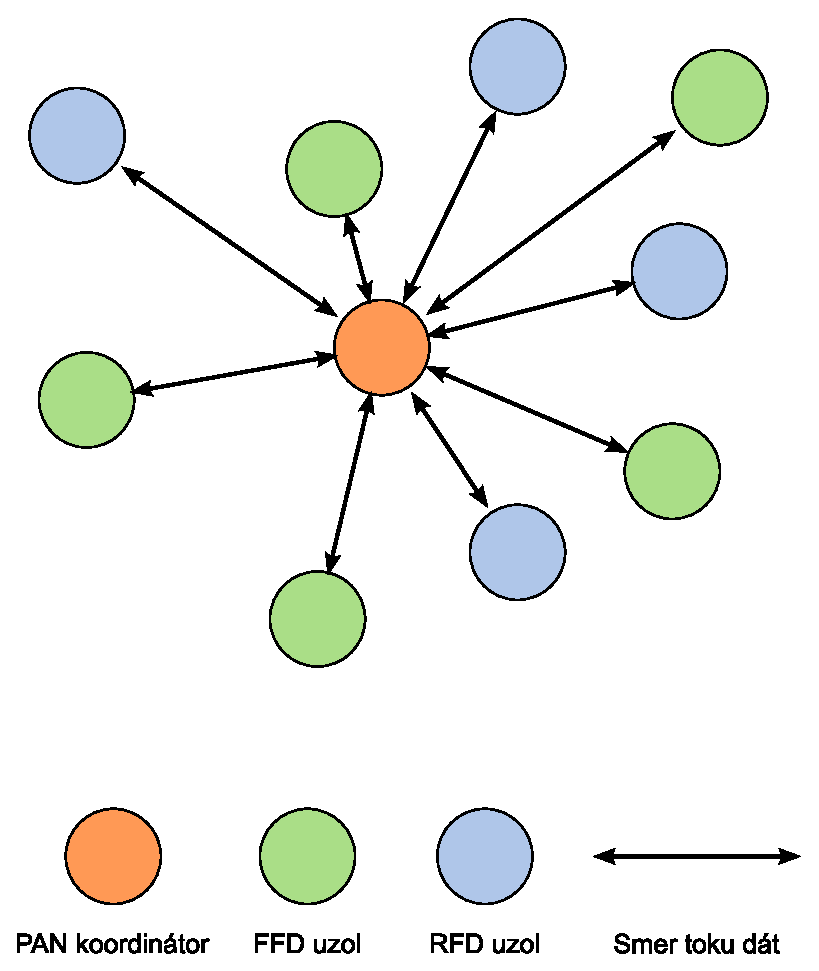
\includegraphics[width=120mm]{figures/topology_star}
\caption{Topológia typu hviezda}
\label{fig:topology_star}
\end{center}
\end{figure} 
\subsubsection{Každý s každým (Peer-to-Peer)}
\indent\indent V tomto type topológie je implementovaná ide aby mohlo každé zariadenie komunikovať s ľubovoľným iným vo svojom dosahu. Takisto v takýchto sieťach existuje jeden FFD prvok v roli PAN koordinátora. Ukážka na obrázku~\ref{fig:topology_p2p}.\\
\begin{figure}[htbp]
\begin{center}
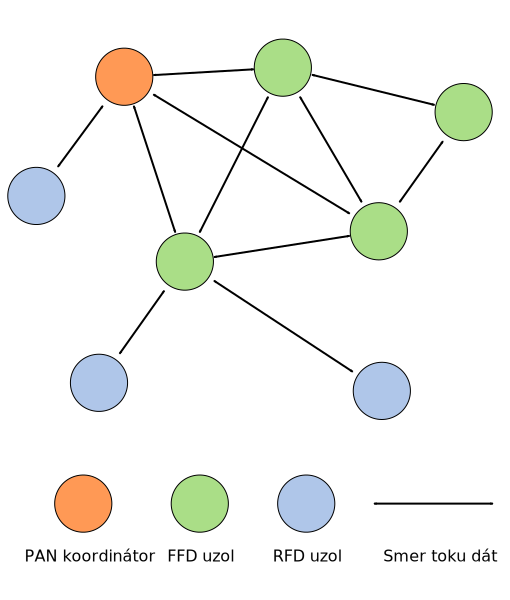
\includegraphics[width=120mm]{figures/topology_p2p}
\caption{Topológia typu každý s každým}
\label{fig:topology_p2p}
\end{center}
\end{figure} 
\indent Z tohoto typu sietí je odvodený variant Zhluk stromov (Cluster Tree). V takejto topológii je prevažná väčšina zariadení typu FFD. Zariadenia typu RFD sa pripájajú k~stromu ako listy. Všetky FFD sú schopné vysielať synchronizačné beacon rámce. Z~nich môže byť však len jeden PAN koordinátor. Ak bude asociácia zariadenia do siete z~nejakého dôvodu odmietnutá, prvok môže vyhľadať iné FFD zariadenie a skúsiť asociáciu u~neho.\\
\indent V prípade, že sú splnené určité podmienky, PAN koordinátor môže požiadať FFD prvok v rámci svojej siete, aby  zformoval novú PAN sieť s novým identifikátorom. Ostatné zariadenia sa potom môžu pripájať až budú tvoriť podobné štruktúry, ako je tá na obr.~\ref{fig:topology_cluster}. Volá sa zhluk stromov (Cluster Tree) Takáto konfigurácia ponúka plošne široké pokrytie, na druhú stranu však správy pri prechode cez viaceré PAN zvyšujú svoju latenciu.\\
\begin{figure}[htbp]
\begin{center}
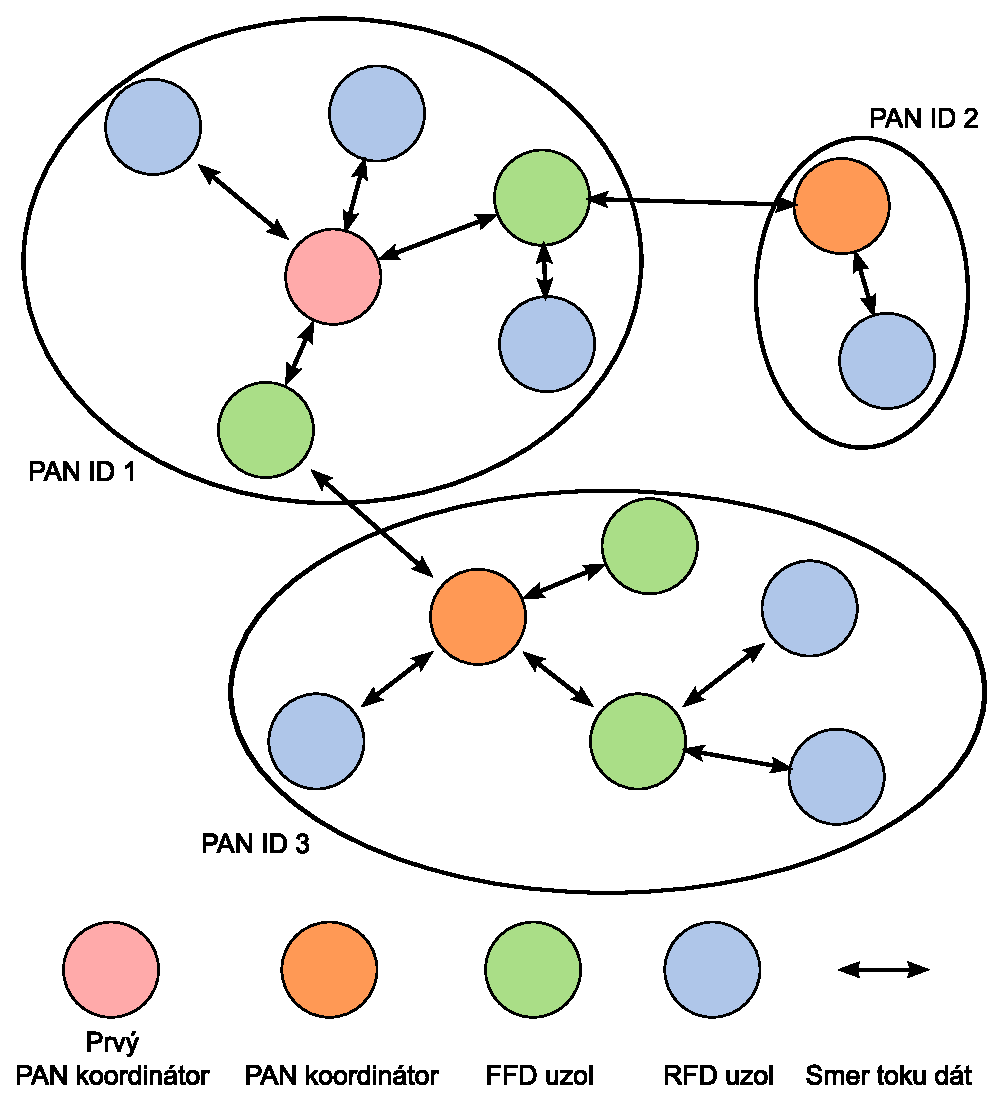
\includegraphics[width=120mm]{figures/topology_cluster}
\caption{Topológia typu zhluk stromov}
\label{fig:topology_cluster}
\end{center}
\end{figure} 
\subsection{Fyzická vrstva}
\indent\indent Ako už bolo spomenuté, jedná sa o technológiu pracujúcu so vzduchom ako zdieľaným médiom. Frekvenčné pásma, v ktorých zariadenia operujú, sú uvedené v tabuľke~\ref{tab:frequencies}. Je vhodné podotknúť, že sa jedná o tzv. bezlicencované (ISM - Industrial Scientific and Medical) pásma, avšak kým 2.4 GHz je s malými obmedzeniami k dispozícii takmer po celom svete, pásmo ISM 868~MHz je len v Európe a ISM 902-928~MHz je k dispozícii len v USA.\\
\begin{table}[htbp]
\begin{center}
\begin{tabular}{|c|c|l|c|c|l|}
  \hline
  \multirow{2}{*}{\textbf{PHY}} & \multirow{2}{*}{\textbf{Frekvencia}} & \multirow{3}{*}{\textbf{Modulácia}} & \textbf{Prenosová} & \textbf{Symbol} & \multirow{3}{*}{\textbf{Symboly}} \\ 
  \multirow{2}{*}{(MHz)} & \multirow{2}{*}{(MHz)} & & \textbf{rýchlosť} & \textbf{rate} & \\ 
  & & & (kbps) & (ksym/s) & \\ [0.5ex]
  \hline\hline
  \multirow{2}{*}{868/915} & 868--868.6 & BPSK & 20 & 40 & Binárne\\
  & 902--928 & BPSK & 40 & 40 & Binárne\\ [0.5ex]
  \hline
  \multirow{2}{*}{868/915} & 868--868.6 & ASK & 250 & 12.5 & 20-bitové PSSS\\
  & 902--928 & ASK & 250 & 50 & 5-bitové PSSS\\ [0.5ex]
  \hline
  \multirow{2}{*}{868/915} & 868--868.6 & O-QPSK & 100 & 25 & 16-kové ortogonálne\\
  & 902--928 & O-QPSK & 250 & 62.5 & 16-kové ortogonálne\\ [0.5ex]
  \hline
  2450 & 2400--2483.5 & O-QPSK & 250 & 62.5 & 16-kové ortogonálne\\ [0.5ex]
  \hline
\end{tabular}
\caption{Používané frekvenčné pásma, modulácie a kódové symboly}
\label{tab:frequencies}
\end{center}
\end{table}
\indent\indent Pre komunikáciu je vyhradených 27 kanálov, ktoré sú združené do troch tzv. stránok kanálov. Takýto spôsob členenia je z historických dôvodov a z dôvodov spätnej kompatibility so zariadeniami fungujúcimi na IEEE 802.15.4-2003. Stránky sú očíslované v rozsahu 0--31, pričom v aktuálne sú stránky 3--31 rezervované do budúcna.\\ 
\indent Na definovanie frekvencie, prenosovej rýchlosti a modulácie je nutné poznať kombináciu hodnoty stránky kanálu a označenie kanálu (z rozsahu 0--26). Pre určenie stránky kanálu je využitých horných 5 bitov (MSB - most significant bit). Pre označenie kanálu sa používa 27-bitová mapa. To znamená, že informácia definujúca potrebné parametre pre komunikáciu na úrovni fyzickej vrstvy sa kompletne obsiahne do 32-bitového identifikátora (viď obr.~\ref{fig:channel_page}). Jednotlivé kombinácie hodnôt stránky kanálov a samotného kanálu sú bližšie rozpísané v tabuľke~\ref{tab:channel_page}.\\
\indent Štandard počíta s tromi základnými typmi modulácie, BPSK (Binary Phase Shift Keying), ASK (Amplitude Shift Keying) a O-QPSK (Offset-Quadrature Phase Shift Keying). PSK (Phase Shift Keying) je modulačná schéma, ktorá transportuje dáta pomocou zmeny fázy referenčného signálu. Jej základná varianta BPSK pracuje s dvoma fázami posunutými o 180 stupňov. To znamená, že jeden kódový symbol reprezentuje jeden bit informácie. Tento spôsob modulácie je relatívne odolný voči rušeniu, ale vyžaduje zložitejšie vysielacie a prijímacie obvody. Hustota informácii na prenesený symbol je nízka, teda je skôr vhodnejší na komunikáciu pri nízkych prenosových rýchlostiach (v prípade 802.15.4 hovoríme o hodnotách 20 a 40 kbps). Alternatívu na frekvenčných pásmach 868/915~MHz predstavil štandard IEEE 802.15.4b-2006, a to použitie ASK modulácie, kedy dáta sú reprezentované variáciami v amplitúde prenášaného signálu. Fáza a frekvencia zostávajú konštantné. Jej princíp je jednoduchý, avšak je citlivá na rušenie, odrazy a pod. ASK nepredstavuje veľmi efektívny spôsob modulácie. Tretí použitý spôsob modulácie datových bitov na nosnú v štandarde IEEE 802.15.4 predstavuje varianta O-QPSK. Pôvodne bol tento typ modulačnej schémy myslený len pre 2.4~GHz ISM pásmo, ale uvedenie tohoto typu modulácie aj pre ostatné frekvenčné pásma, predstavené so štandardom IEEE 802.15.4b-2006, znamenalo zjednodušenie pre koncové prvky, pretože pre prácu v pásmach 868~MHz, 915~MHz a 2.4~GHz potom stačí jeden modulačný a demodulačný obvod. Schéma O-QPSK teda pracuje so štyrmi variáciami posunu fázy (4 stavy), to znamená, že vie na jeden symbol modulovať 2 bity ($2^{2}=4$). Identifikátor \textit{offset} v názve charakterizuje posun pri modulovaní párnych a nepárnych bitov. Tento posun má veľkosť, ktorá predstavuje polovicu dĺžky vysielania jedného symbolu. Dochádza k posunu fázy vždy len o 90 stupňov, čo zabraňuje skokovým zmenám amplitúdy. Táto \textit{offset} varianta kvadratúrnej fázovej modulácie je často preferovaná.\\
\begin{figure}[htbp]
\begin{center}
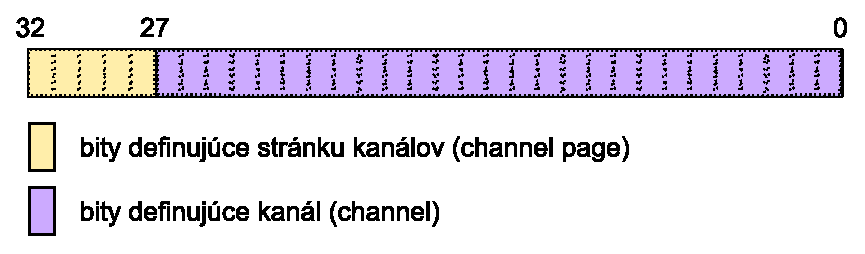
\includegraphics[width=120mm]{figures/channel_page}
\caption{32-bitový identifikátor kanálov a stránky kanálov}
\label{fig:channel_page}
\end{center}
\end{figure}
\begin{table}[htbp]
\begin{center}
\begin{tabular}{|c|c|c|c|c|}
  \hline
  \textbf{Stránka kanálu} & \textbf{Stránka kanálu} & \textbf{Číslo kanálu} & \textbf{Frekvenčné} & \\
  (dekadicky) & (binárne) & (dekadicky) & \textbf{pásmo} & \raisebox{1.5ex}{\textbf{Modulácia}} \\
  \hline
  \hline
  \multirow{3}{*}{0} & \multirow{3}{*}{0 0 0 0 0} & 0 & 868 MHz & BPSK \\
  \cline{3-5}
  & & 1--10 & 915 MHz & BPSK \\
  \cline{3-5}
  & & 11--26 &  2.4 GHz & O-QPSK \\ [0.5ex]
  \hline
  \multirow{3}{*}{1} & \multirow{3}{*}{0 0 0 0 1} & 0 & 868 MHz & ASK \\
  \cline{3-5}
  & & 1--10 & 915 MHz & ASK \\
  \cline{3-5}
  & & 11--26 & \multicolumn{2}{|c|}{Rezervované} \\ [0.5ex]
  \hline
  \multirow{3}{*}{2} & \multirow{3}{*}{0 0 0 1 0} & 0 & 868 MHz & O-QPSK \\
  \cline{3-5}
  & & 1--10 & 915 MHz & O-QPSK \\
  \cline{3-5}
  & & 11--26 & \multicolumn{2}{|c|}{Rezervované} \\ [0.5ex]
  \hline
  3--31 & 0 0 0 1 1 -- 1 1 1 1 1 & \multicolumn{3}{|c|}{Rezervované} \\ [0.5ex]
  \hline
\end{tabular}
\caption{Zoznam jednotlivých kombinácii kanálov, frekvenčných pásiem a použitých modulácii podľa nastavenia identifikátorov kanálov a stránky kanálov}
\label{tab:channel_page}
\end{center}
\end{table}
\subsection{Linková vrstva}
\indent\indent Linková vrstva IEEE 802.15.4b podľa~\cite{ieee06} je jednoduchá, ale flexibilná. Riadi a kontroluje prístup k zdieľanému médiu. K tomuto využíva nasledovné mechanizmy:
\begin{itemize}
\item Vysielanie beacon rámcov (periodicky, alebo neperiodicky v závislosti od aktuálnej konfigurácie siete)
\item Synchronizácia podľa beacon rámcov vysielaných svojimi susedmi
\item Podieľanie sa na procesoch asociácie a disasociácie v PAN sieti
\item V prípade požiadavku, podpora zabezpečenia
\item Prístup k médiu pomocou CSMA-CA algoritmu
\item Riadi a prideľuje GTS časové sloty 
\end{itemize}
\subsection{Beaconing a non-beaconing módy}
\indent\indent  Linková vrstva môže pracovať v dvoch základných režimoch - tzv. beaconing mód a~non-beaconing mód. Rozdiel medzi týmito módmi nie je v tom, či sú beacon rámce v~sieti posielané, ale v tom, či sú tieto rámce posielané pravidelne. V prípade, že je hodnota atribútu u koordinátora siete $macSuperframeOrder < macBeaconOrder$, to znamená, že sieť pracuje v beaconing móde a beacon rámce sú posielané pravidelne v~intervale vypočítanom podľa vzťahu 
$$ beaconPeriod = aBaseSuperframeDuration * 2^{macBeaconOrder}$$
kde výsledná hodnota intervalu je v symboloch. Podľa tabuľky~\ref{tab:frequencies} sa táto hodnota dá previesť na čas v sekundách. Hodnota konštanty aBaseSuperframeDuration je $960$ a~predstavuje dĺžku najkratšieho možného intervalu v symboloch oddeľujúceho začiatky dvoch beacon rámcov.\\
\indent Alternatívu predstavujú zhodné hodnoty atribútov \textit{macBeaconOrder} a \textit{macSuperframeOrder}. Vtedy sa jedná o non-beaconing mód a beacon rámce sa posielajú len ako odpoveď na explicitnú požiadavku o ich zaslanie.\\
\subsection{Superframe rámec}
\indent\indent Nami navrhovaný model uvažuje použitie beaconing módu, ktorý ponúka zaujímavejší mechanizmus komunikácie a využíva možnosti dané periodicitou v zasielaní riadiacich a kontrolných beacon rámcov. V tomto beaconing móde sa využíva komunikačná štruktúra, ktorá sa nazýva superframe rámec. Superframe rámec vymedzuje 4 periodicky sa opakujúce úseky (obr.~\ref{fig:superframe}) a pre každý z nich platia pravidlá pre posielanie a príjem dát. Superframe rámec vždy obsahuje 16 superframe slotov o dĺžke $aBaseSlotDuration * 2^{macSuperframeOrder}$ symbolov dynamicky distribuovaných do Contention Access periódy a Contention Free periódy. Slot, v ktorom je vysielaný beacon rámec je označovaný ako slot 0. Konštanta \textit{aBaseSlotDuration} má hodnotu $60$.\\
\begin{figure}[htbp]
\begin{center}
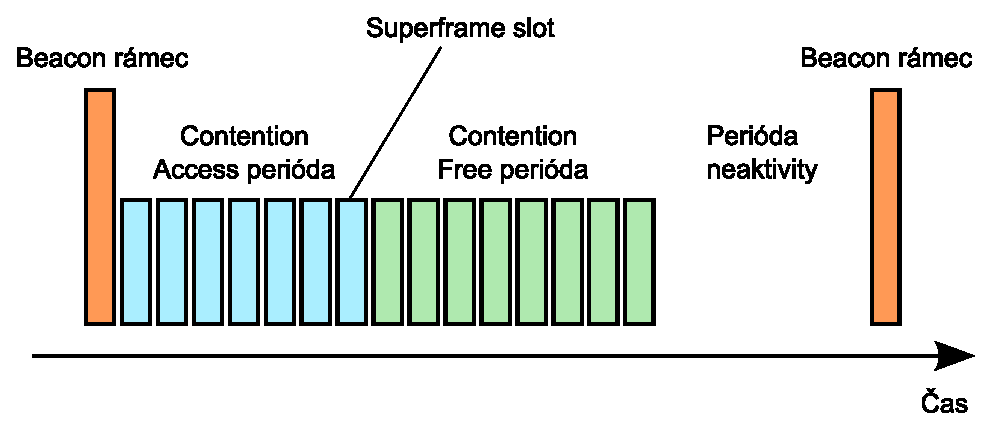
\includegraphics[width=140mm]{figures/superframe}
\caption{Štruktúra superframe rámca (obrázok nie je v mierke)}
\label{fig:superframe}
\end{center}
\end{figure}
\subsubsection{Beacon rámec}
\indent\indent Na úvod každého superframe rámca je FFD prvkom, ktorý je v sieti pripojený ako smerovač (router), posielaný beacon rámec. Obsahuje informačné polia, ktoré okrem iného obsahujú atribúty \textit{macBeaconOrder} a \textit{macSuperframeOrder} definujúce isté vlastnosti danej PAN siete. Z týchto polí vychádzajú hraničné časovače určujúce dĺžky jednotlivých úsekov superframe rámca. Okrem toho definuje aj koniec Contention Access periódy pomocou identifikátora \textit{FinalCAPSlot}.\\
\indent Beacon rámec je vysielaný prvkom bez použitia CSMA metódy, pretože všetky prvky v dosahu vysielača daného FFD prvku by sa mali synchronizovať na periodicitu týchto rámcov a nevysielať žiadne dáta na prenosové médium v čase, keď sa očakáva beacon rámec.\\
\paragraph{Contention Access perióda}
Počas tejto periódy prvky môžu pristupovať na médium pomocou metódy CSMA-CA. Tento moment slúži hlavne na vybavovanie žiadosti o asociáciu do siete, prípadne žiadosti o prenos užitočných dát smerom od FFD prvku. V takom prípade sú dáta, ktoré chce FFD poslať svojim susedom indikované v beacon rámci. FFD prvky majú väčšinou fronty na zasielanie týchto rámcov s užitočnými dátami pre koncové zariadenia. Ak si sused daného smerovača nevyžiada dáta po uplynutí nejakého konkrétneho počtu superframe rámcov od ich prvého indikovania v beacon rámci, smerovač ich z tejto fronty zahadzuje.\\
\indent Prvok, ktorému smerovač v beacon rámci neindikoval, že má pre neho vo svojich frontách zaradené dáta, a tento prvok ani nemá záujem žiadne dáta poslať smerom k~FFD zariadeniu môže vypnúť svoje vysielacie a prijímacie obvody a šetriť tak energiu.\\
\paragraph{Contention Free perióda}
Časový interval v ktorom sa prenášajú dáta pomocou mechanizmu GTS (Guaranteed Time Slot) sa nazýva Contention Free perióda. GTS mechanizmus alokuje určitý počet superframe slotov pre prenos dát, ktoré často majú periodický charakter. Beacon rámec posielaný smerovačom na úvod superframe rámca definuje aj počet alokovaných superframe slotov združených do GTS slotov a pre každý z týchto GTS slotov pomocou 16-bitovej, alebo 64-bitovej adresy určí druhú stranu komunikačného toku. Pomocou jednoduchej bitovej mapy je následne určený smer komunikácie (smerom od smerovača/smerom k smerovaču). GTS mechanizmus je v novom štandarde IEEE 802.15.4b-2006 vedený už len ako dobrovoľný spôsob prístupu k prenosu dát.\\

\section{ZigBee}
\indent\indent Medzi štandardy definujúce vyššie vrstvy komunikácie v LR-WPAN sieťach patrí napríklad ZigBee od združenia ZigBee Alliance~\cite{zigbee08}. Tento štandard definuje sieťovú a~aplikačnú vrstvu siete ZigBee a v prípade linkovej a sieťovej vrstvy sa spolieha na už vyššie popísaný štandard IEEE 802.15.4. Vzťah medzi ZigBee a IEEE 802.15.4 by sa dal prirovnať vzťahu medzi Wi-Fi a IEEE 802.11. Na obr.~\ref{fig:zigbee_ieee} je vyobrazený vzťah medzi vrstvami definovanými v ZigBee a IEEE štandardoch. Prvá z finálnych verzii ZigBee štandardu sa objavila koncom roku 2004, ale odvtedy bola ešte niekoľko krát upravovaná. My v tomto dokumente pracujeme s verziou z januára 2008~\cite{zigbee08}, momentálne najaktuálnejšou.\\
\begin{figure}[htbp]
\begin{center}
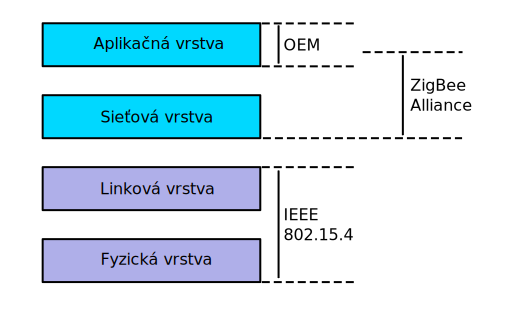
\includegraphics[width=140mm]{figures/zigbee_ieee}
\caption{Vzťah medzi ZigBee Alliance a IEEE 802.15.4}
\label{fig:zigbee_ieee}
\end{center}
\end{figure}
\indent Svojou charakteristikou sú siete ZigBee vhodné pre aplikácie nevyžadujúce vysoké nároky na datovú priepustnosť, uspokoja sa s bezdrôtovým spojením krátkeho dosahu, ale hlavne pre ktoré je kritická nízka energetická náročnosť. Tieto špecifiká posúvajú sie\-te ZigBee ako vhodného kandidáta pre bezdrôtové riadenie osvetlenia, termoreguláciu, bezpečnostné prvky v inteligentných domácnostiach, pre komunikáciu hlásičov požiaru v budovách, alebo aj v medicíne pre rýchle predávanie správ o stave pacienta do definovaného zberného bodu. V priemysle by zase táto technológia našla využitie napríklad v monitorovaní podmienok, v akých sa tovar nachádza v sklade (teplota, vlhkosť, vibrácie), alebo napríklad pri kontrole procesov v čističke odpadových vôd. Keďže sieť má vlastnosť samokonfigurácie, jej inštalácia aj vo väčších mierkach je otázkou zopár hodín.\\
\subsection{Architektúra ZigBee}
\indent\indent Architektúra siete ZigBee sa skladá zo štyroch základných vrstiev, ako zobrazuje aj obr.~\ref{fig:zigbee_ieee}. Tieto vrstvy medzi sebou komunikujú predávaním správ cez tzv. body prístupu služby (SAP - Service Access Point). SAP je v princípe miesto, v ktorom jedna v vrstiev môže požadovať služby druhej vrstvy. štruktúra architektúry spolu s vyznačenými SAP bodmi je vyobrazená na obrázku~\ref{fig:architecture_zigbee}. Na ňom môžme rozlišovať dva typy SAP bodov medzi jednotlivými vrstvami. Jeden typ predstavujú body, cez ktoré sú spracovávané užitočné dáta aplikácii (napr. MCPS-SAP, alebo PD-SAP) a druhý typ SAP bodov sa zaoberá manažmentom siete, ako napr. konfigurácia beacon rámcov, prípadne nastavovanie, alebo čítanie hodnôt atribútov (napr. MLME-SAP, PLME-SAP body).\\
\begin{figure}[htbp]
\begin{center}
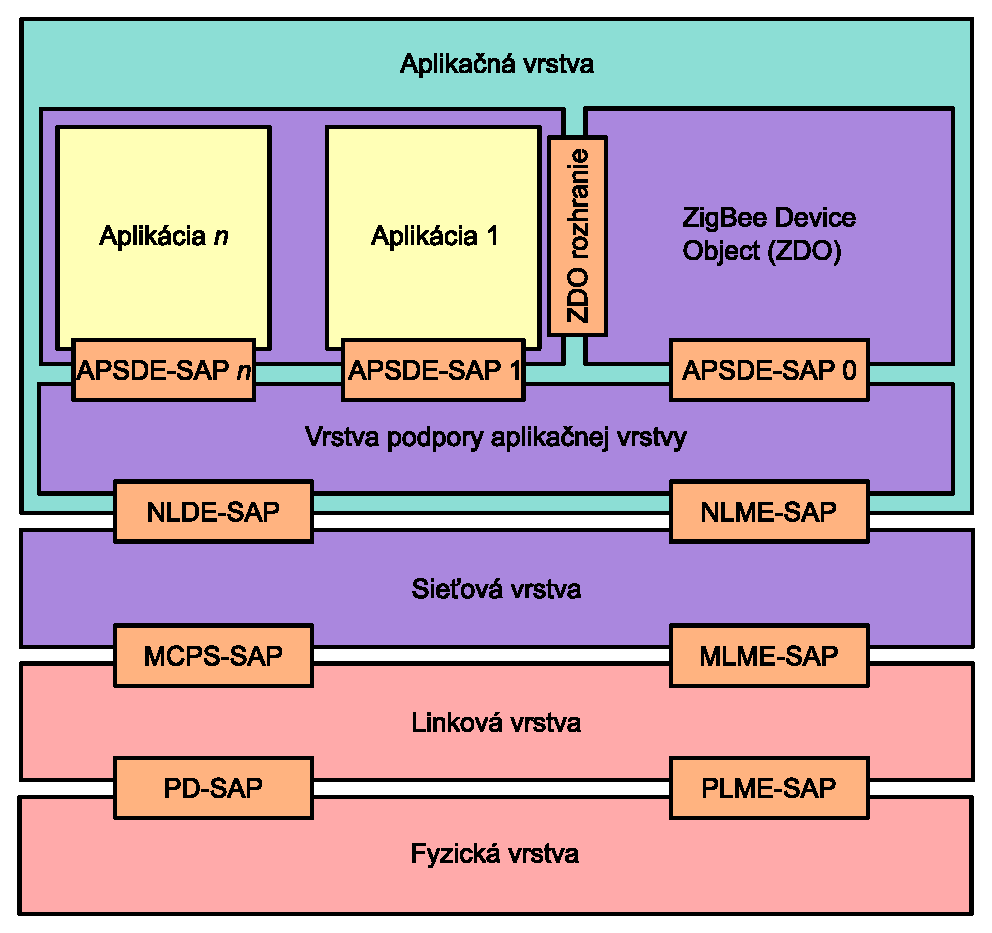
\includegraphics[width=140mm]{figures/architecture_zigbee}
\caption{Znázornenie vrstvovej architektúry siete ZigBee}
\label{fig:architecture_zigbee}
\end{center}
\end{figure}
\subsection{Sieťová vrstva}
\indent\indent Požiadavky na sieťovú vrstvu sú zabezpečovanie správneho fungovania linkovej vrstvy a poskytovania vhodných služieb vyššie postavenej aplikačnej vrstve. Podľa konceptu, sieťová vrstva obsahuje dve entity, ktorých služby sú využívané aplikačnou vrstvou. Tie\-to entity sú datová (NLDE - NWK Layer Data Entity) a manažement entita (NLME - NWK Layer Management Entity). Ku každej sa pristupuje cez príslušný bod SAP - NLDE-SAP, alebo NLME-SAP. Zmysel rozdelenia sieťovej vrstvy na tieto dve časti je v~tom, že NLME využíva NLDE pre vykonávanie potrebných úloh, ktoré majú charakter riadenia a kontroly na danej úrovni a takisto zabezpečuje prístup k sieťovej informačnej databázy (NIB - Network Information Base).\\
\subsection{Aplikačná vrstva}
\indent\indent Ako je ukázané na obrázku~\ref{fig:architecture_zigbee}, aplikačná vrstva sa skladá zo ZigBee Device Object objektu, z aplikačných objektov (definovaných výrobcom zariadenia, alebo aplikácie) a~z~podpornej vrstvy APS.\\
\subsubsection{Podporná vrstva aplikačnej vrstve}
\indent\indent Uvedená vrstva je v špecifikácii označovaná ako APS (Application Support Sub\-layer). Úlohy, ktoré jej prináležia si delia dve entity: datová (APSDE) a manažment (APSME). Datová ma na starosť sprístupnenie služieb pre aplikačné vrstvy v danej sieti a management entita zabezpečuje cez príslušný SAP bod funkcie bezpečnosti prenosu, prípadne prístup k informačnej báze danej podvrstvy. S podobným rozdelením sa budeme stretávať aj pri ostatných vrstvách protokolu.\\
\subsubsection{Objekty typu ZigBee Device Objects}
\indent\indent ZigBee Device Objects objekty (ZDO) hrajú dôležitú úlohu v protokole ZigBee. Pri štarte siete inicializujú sieťovú vrstvu a vrstvu APS. Na základe požiadavkov aplikácii dávajú impulz k procesom, ktoré realizujú vytváranie PAN, asociáciu do už existujúcej siete PAN, prípadne majú na starosť správu sieťovej vrstvy. Ako už bolo spomenuté v~\cite{halas03} ZDO môžme nazvať komunikačným bodom aplikačnej vrstvy. ZDO poskytuje funkcie pre všetky aplikácie bežiace na ZigBee zariadení vrátane skenovania siete (device and service discovery), vytvorenia spojení medzi objektami v sieti (binding) a správy šifrovacích kľúčov (security management). Vo výslednej simulácii je jediná z jej úloh inicializácia daného zariadenia spolu s nastavením základných parametrov pre spojenie. Na aplikačnej vrstve sú uvažované tzv. endpoints. Zariadenie môže mať nadefinovaných max. 240 endpoints a každému z nich zodpovedá jeden aplikačný profil. Pre ilustráciu môžme uviesť, že cez jeden endpoint je realizovaná komunikácia s cieľom zapnúť svetlo a cez iný endpoint môže aplikácia informovať iný ZigBee prvok o teplote prostredia zmeranej teplotným čidlom.\\
\subsection{Väzba na IEEE 802.15.4}
\indent\indent V špecifikácii k IEEE 802.15.4 sú uvedené aj doplnkové podvrstvy k základnéj vrstvovej štruktúre. Na mysli máme podvrstvy označované ako SSCS (Sublayer-Specific Convergence Layer) a LLC (Logical Link Control) vrstvy. Ich polohu znázorňuje obrázok~\ref{fig:architecture_sublayers}. Konvergenčná SSCS vrstva slúži k predávaniu informácii medzi sieťovou a~linkovou vrstvou. Následne má schopnosť informovať nadradené vrstvy o tom, v akom stave sa nachádza posielanie dát ostatným členom siete. Funkciou podvrstvy IEEE 802.2 LLC  je kontrola a zaistenie integrity dátových prenosov. LLC vrstva poskytuje cez body prístupu (SAP) služby linkovej vrstvy pre sieťovú vrstvu.\\
\begin{figure}[htbp]
\begin{center}
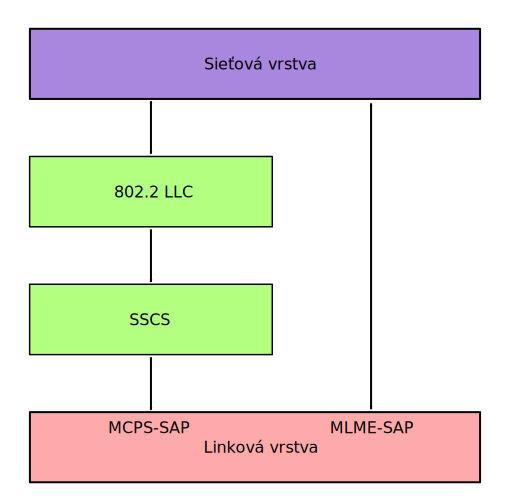
\includegraphics[width=120mm]{figures/architecture_sublayers}
\caption{Použitie doplňujúcich vrstiev v komunikácii medzi linkovou a sieťovou vrstvou}
\label{fig:architecture_sublayers}
\end{center}
\end{figure}